\documentclass[]{article}
\usepackage[utf8]{inputenc}
\usepackage{amsmath}
\usepackage{graphicx}
\usepackage{cleveref}

\title{Error function}
\author{Hasse Hansen}
\date{March 2019}

\begin{document}

\maketitle

 
\section{Introduction}
This report gives a small introduction to the error function and its properties along side containing a plot of the error function. 

The name of the error function originates from J.W.L. Glaisher, who in 1871 connected it to "the theory of Probability, and notably the theory of Errors".

The error function is a function used in error theory and probability. The function is defined as: 
\begin{align}
    \mathrm{erf}(x) &= \frac{1}{\sqrt{\pi}} \int_{-x}^x \exp{-t^2} dt  \nonumber\\
    &=  \frac{2}{\sqrt{\pi}} \int_{0}^x \exp{-t^2} dt.
    \label{eq:definition}
\end{align}
It describes the probability of a random variable, Y, having a value between $-x$ and $x$ - with the assumptions that Y is normal distributed with a mean of 0 and variance of 0.5. To see a plot of the error function, see \cref{fig:Error}.

\section{Properties of the error function}
The error function has the property of 
\begin{equation}
    \mathrm{erf}(-x) = -\mathrm{erf}(x)
\end{equation}
since the error function is an odd function. This property originates in the integrand in \cref{eq:definition}, since $\exp{-t^2}$ is a even function.

Additionally for a complex number z, it also holds that
\begin{equation}
    \mathrm{erf}(\Bar{z}) = \overline{\mathrm{erf}(z)}
\end{equation}
where $\Bar{z}$ is the complex conjugated of z.

The error function is an entire function, which only has singularities at infinity, at the value of 1. The Taylor expansion of the error function always converges.

\begin{figure*}
    \centering
    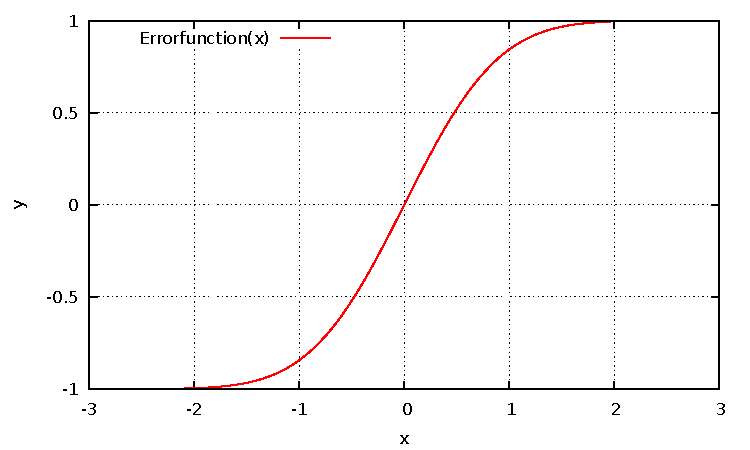
\includegraphics{Error_plot.pdf}
    \caption{A plot of the error function as a function of x, with x ranging from -3 to 3. }
    \label{fig:Error}
\end{figure*}


\end{document}
